\documentclass{UTNetLab}

\usepackage{graphicx}

\title{Static and Dynamic Routing}
\newcommand\reference{
	S. S. Panwar, S. Mao, J.-dong Ryoo, and Y. Li, “Static and dynamic routing,” in TCP/IP Essentials: A Lab-Based Approach, Cambridge: Cambridge University Press, 2004, pp. 77–99.
}

\begin{document}
	\section*{Objectives}
	\begin{itemize}
		\item Comparison of router and bridge.
		\item IP forwarding.
		\item Use of ICMP messages in routing.
		\item The Routing Information Protocol (RIP).
		\item The Open Shortest Path First (OSPF) protocol.
		\item Static routing by manually building the routing tables in the routers and hosts.
		\item Use of \textbf{Traceroute} to find an end-to-end route.
	\end{itemize}
	
\part{A Simple Router Experiment}
In this lab, you need two hosts, a bridge, and two hubs, which are required to be connected as shown in \hyperref[tab:4.2]{Table~4.2} and \hyperref[tab:4.3]{Table~4.3}.
    \begin{table}[H]
        \caption{Router and Host IP addresses for \hyperref[fig:4.10]{Figure~4.10} (Table~4.2\label{tab:4.2}, Table~4.3\label{tab:4.3})}
        \centering
        \begin{tabular}{ *2c | *2c | *2c }
            \hline \hline
            \multicolumn{2}{c|}{Router} & \multicolumn{2}{c|}{Host\textsubscript{A}} & \multicolumn{2}{c}{Host\textsubscript{B}} \\
            f0/0 & f1/0 & Name & IP Address & Name & IP Address \\
            \hline 
            128.238.61.1/24 & 128.238.62.1/24 & h0 & 128.238.61.101/24 & h1 & 128.238.62.101/24 \\
            % 2 & 128.238.62.2/24 & 128.238.63.2/24 & h2 & 128.238.62.102/24 & h3 & 128.238.63.102/24 \\
            % 3 & 128.238.63.3/24 & 128.238.64.3/24 & h4 & 128.238.63.103/24 & h5 & 128.238.64.103/24 \\
            % 4 & 128.238.64.4/24 & 128.238.65.4/24 & h6 & 128.238.64.104/24 & h7 & 128.238.65.104/24 \\
            \hline \hline
            \end{tabular}
    \end{table}

    \begin{figure}[H]
        \centering
        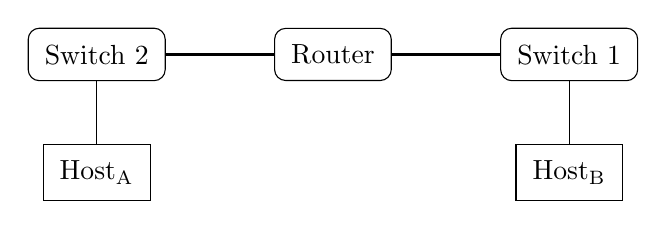
\begin{tikzpicture}[every node/.style={inner sep=6}]
            \node[draw] (h1) at (-3,-1.5){Host\textsubscript{A}};
            \node[draw,rounded corners] (hub2) at (-3,0){Switch 2};
            \node[draw,rounded corners] (router) at (0,0){Router};
            \node[draw,rounded corners] (hub1) at (3,0){Switch 1};
            \node[draw] (h0) at (3,-1.5){Host\textsubscript{B}};
        
            \draw (h0) -- (hub1);
            \draw (h1) -- (hub2);
            \draw[thick] (hub1) -- (router);
            \draw[thick] (hub2) -- (router);
        \end{tikzpicture}
        \caption{Simple router experiment (Figure~4.10)}\label{fig:4.10}
    \end{figure}

\section{Simple Routing}

    Configure the IP addresses of your hosts and the router as shown in \hyperref[fig:4.10]{Figure~4.10}, \hyperref[tab:4.2]{Table~4.2} and \hyperref[tab:4.3]{Table~4.3} (select one of row in table).
    
    \textbf{Note:} in Figure 4.10 that we've provided for you, the above topology is configured.

    Initially all hosts’ routing table has no entry for the subnet on the other side of the router.
    In order to be connected, you need to add a routing entry for the other subnet in the routing table of all hosts (see section 4.3.1).

    You can use one of the following commands to add routing in hosts.
    
    \lstset{backgroundcolor=\color{green!10}}
    \begin{lstlisting}
# by ip command
ip route add remote-subnet dev eth1            # with interface name
ip route add remote-subnet via gateway-ip    # with default gateway
# or by route command
route add -net remote-subnet dev eth1           # with interface name
route add -net remote-subnet gw gateway-ip   # with default gateway
    \end{lstlisting}
    \begin{itemize}
        \item \textit{remote-subnet} is a subnet ip with mask number. It must be like \lstinline{128.238.62.0/24}.
        \item \textit{gateway-ip} is a gateway ip in your network. It must be like \lstinline{128.238.61.1}
        \item \textit{eth1} is a pyhisical interface name. It is shown in \lstinline{ifconfig} or \lstinline{ip a} commands.
    \end{itemize}
    
    \textbf {\textit{Note:} for example, enter the below commands in \textit{h0} and \textit{h1}'s Console: }
    
    \fcolorbox{blue}{red!10}{{h\textsubscript{0}}'s Console}
    \lstset{backgroundcolor=\color{red!10}}
    \begin{lstlisting}
    ip route add 128.238.62.0/24 dev eth1
    \end{lstlisting}

    \fcolorbox{blue}{red!10}{{h\textsubscript{1}}'s Console}
    \lstset{backgroundcolor=\color{red!10}}
    \begin{lstlisting}
    ip route add 128.238.61.0/24 dev eth1
    \end{lstlisting}
    
    Run \lstinline{wireshark} on the first machine and also on the second machine in the other subnet simultaneously:
    
    
    \fcolorbox{blue}{lime!30}{{h\textsubscript{0} and h\textsubscript{1}}'s Wireshark}
    \lstset{backgroundcolor=\color{lime!30}}
    \begin{lstlisting}
    Run wireshark on eth1, Filter: ip.addr == 128.238.61.101 && ip.addr == 128.238.62.101
    \end{lstlisting}
    
    Send \lstinline{ping} messages continuously to the other machine:
    
    \fcolorbox{blue}{red!10}{{h\textsubscript{0}}'s Console}
    \lstset{backgroundcolor=\color{red!10}}
    \begin{lstlisting}
    ping -sv 128.238.62.101
    \end{lstlisting}
    
    After receiving the tenth echo reply, quit \lstinline{ping} and save the \lstinline{wireshark} outputs of both machines.
    Also, copy the \lstinline{ping} output.

    During this exercise, don’t run the \lstinline{ping} program at the same time.
    For clean results, do your experiments in turn.
    
    \begin{report}
    \item When a packet was sent to a host in the other subnet, explain how the source and destination Ethernet addresses were changed.
    
    \item What are the source and destination addresses in the IP and Ethernet headers of a packet that went from your machine to the router?
    
    \item What are the source and destination addresses in the IP and Ethernet headers of a packet that went from the router to your partner’s machine?
    
    \item Answer the above two questions, but now for the echo reply that was returned from your partner’s machine.

    \item Use the \lstinline{wireshark} outputs from both machines to calculate the average delay that a packet experienced in the router. Note that the system times of the two machines might be different. Show all the steps and submit the \lstinline{wireshark} outputs with your report.
    
    \item Compare this value with the previous value in the case of the bridge. Which, a router or a bridge, is faster? Why?
    \end{report}

\part{RIP Exercises}\label{sec:rip}
   
    Consider \hyperref[fig:4.11]{Figure~4.11} as our network topology for this section.
    
    In this section, we will examine the operation of RIP. To enable the RIP routing process in a router, you can use the following commands in the \textit{Global Configuration} mode (use \lstinline[language={cisco}]{enable} command first if needed).
  
     \fcolorbox{blue}{green!10}{{R\textsubscript{1}\#}}
    \lstset{backgroundcolor=\color{green!10}}
    \begin{lstlisting}[frame=trBL,language={cisco}]
    config term
    R1(config)# router rip
    R1(config-router)# network network-number
    \end{lstlisting}
     
    where \textit{network-number} could be 128.238.0.0 (Note: this means that you must replace \textit{network-number} with 128.238.0.0 in above command).
    
    \textbf{Note: }You should repeat the above commands for all routers.
    
    To remove the network, you can use:
        
    \fcolorbox{blue}{green!10}{{R\textsubscript{1}(config-router)\#}}
    \lstset{backgroundcolor=\color{green!10}}
    \begin{lstlisting}[frame=trBL]
    no network network-number
    \end{lstlisting}
    To shutdown the RIP process, you can use:
    
    \fcolorbox{blue}{green!10}{{R\textsubscript{1}(config)\#}}
    \lstset{backgroundcolor=\color{green!10}}
    \begin{lstlisting}[frame=trBL]
    no router rip
    \end{lstlisting}
   

    % You can see router RIP status and state by following command in router \textit{Privileged EXEC} mode.
    % \begin{itemize}
    %     \item \lstinline[language={cisco}]{show ip rip [,route,interface,statistics]}
    % \end{itemize}
    
    % Since the IP address of \textit{ethernet1} in \textit{router4} is the only interface which is different from the initial configuration in Appendix~B of reference book, we will reboot all the four routers to restore their default configurations, and change the IP address on the \textit{ethernet1} in \textit{router4} only. Since our hosts started \lstinline{routed} at boot-up time, no further action is needed to run RIP on the hosts. \footnote{The lab instructor should make sure that the IP-Forwarding function is enabled in each host.}
    Configure network routers and hosts as \hyperref[fig:4.11]{Figure~4.11}. Since our hosts don’t have \lstinline{routed} package, you need to add route for subnet \textit{128.238.0.0/16} to each host.
    
     \fcolorbox{blue}{red!10}{{h\textsubscript{i}}'s Console , i $\in$ \{0,1,...,7\}}
    \lstset{backgroundcolor=\color{red!10}}
    \begin{lstlisting}
    ip route add 128.238.0.0/16 dev eth1
    \end{lstlisting}
    
    \begin{figure}[H]
        \centering
        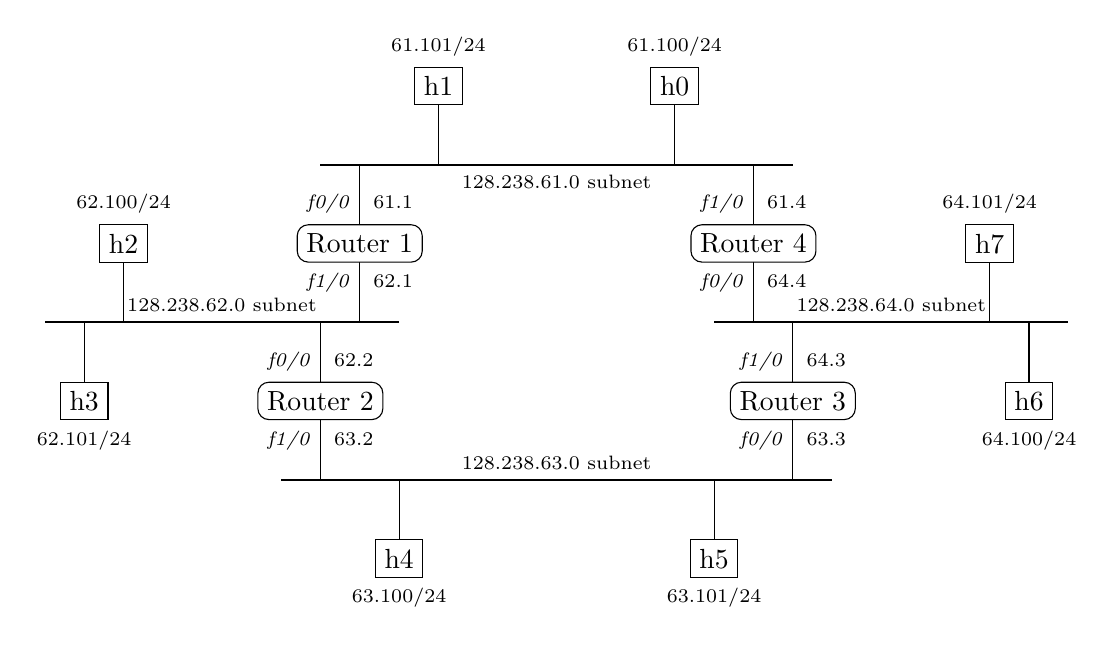
\begin{tikzpicture}
            \draw (2.5,1) node[draw,fill=white,rounded corners] (br4) {Router 4}
                -- +(0,-1)
                -- +(0,+1)
                +(0,0.5) node {\scriptsize\textit{f1/0}\quad 61.4}
                +(0,-0.5) node {\scriptsize\textit{f0/0}\quad 64.4}
            ;
            \draw (3,-1) node[draw,fill=white,rounded corners] (br3) {Router 3}
                -- +(0,-1)
                -- +(0,+1)
                +(0,0.5) node {\scriptsize\textit{f1/0}\quad 64.3}
                +(0,-0.5) node {\scriptsize\textit{f0/0}\quad 63.3}
            ;
            \draw (-2.5,1) node[draw,fill=white,rounded corners] (br1) {Router 1}
                -- +(0,-1)
                -- +(0,+1)
                +(0,0.5) node {\scriptsize\textit{f0/0}\quad 61.1}
                +(0,-0.5) node {\scriptsize\textit{f1/0}\quad 62.1}
            ;
            \draw (-3,-1) node[draw,fill=white,rounded corners] (br2) {Router 2}
                -- +(0,-1)
                -- +(0,+1)
                +(0,0.5) node {\scriptsize\textit{f0/0}\quad 62.2}
                +(0,-0.5) node {\scriptsize\textit{f1/0}\quad 63.2}
            ;
            \draw (5.5,1) node[draw,fill=white] {h7}
                -- +(0,-1)
                +(0,0.5) node {\scriptsize 64.101/24}
            ;
            \draw (6,-1) node[draw,fill=white] {h6}
                -- +(0,1)
                +(0,-0.5) node {\scriptsize 64.100/24}
            ;
            \draw (-5.5,1) node[draw,fill=white] {h2}
                -- +(0,-1)
                +(0,0.5) node {\scriptsize 62.100/24}
            ;
            \draw (-6,-1) node[draw,fill=white] {h3}
                -- +(0,1)
                +(0,-0.5) node {\scriptsize 62.101/24}
            ;
            \draw (-1.5,3) node[draw,fill=white] {h1}
                -- +(0,-1)
                +(0,0.5) node {\scriptsize 61.101/24}
            ;
            \draw (1.5,3) node[draw,fill=white] {h0}
                -- +(0,-1)
                +(0,0.5) node {\scriptsize 61.100/24}
            ;
            \draw (-2,-3) node[draw,fill=white] {h4}
                -- +(0,1)
                +(0,-0.5) node {\scriptsize 63.100/24}
            ;
            \draw (2,-3) node[draw,fill=white] {h5}
                -- +(0,1)
                +(0,-0.5) node {\scriptsize 63.101/24}
            ;
            \draw[thick] (2,0) -- +(4.5,0) node[pos=0.5,above] {\scriptsize 128.238.64.0 subnet};
            \draw[thick] (-2,0) -- +(-4.5,0) node[pos=0.5,above] {\scriptsize 128.238.62.0 subnet};
            \draw[thick] (-3,2) -- +(6,0) node[pos=0.5,below] {\scriptsize 128.238.61.0 subnet};
            \draw[thick] (-3.5,-2) -- +(7,0) node[pos=0.5,above] {\scriptsize 128.238.63.0 subnet};
        \end{tikzpicture}
        \caption{Network Configuration for \nameref{sec:rip} (Figure~4.11)}\label{fig:4.11}
    \end{figure}
\section{RIP Messages}
    Connect the routers and hosts and change the IP addresses of the hosts and routers as shown in \hyperref[fig:4.11]{Figure~4.11}.
    
     \textbf{Note:} in Figure 4.11 that we've provided for you, the above topology is configured.
     
    Also, make sure that your host does not have other routing entries than your own subnet and your loopback interface.
    For how to remove an entry from the host routing table, see Section~4.3 of the reference book.

    Configure the RIP in each router. For this purpose, enter the following commands for all routers (use \lstinline[language={cisco}]{enable} command first if needed).
    
         \fcolorbox{blue}{yellow!10}{{R\textsubscript{i}\# , i $\in$ \{1,...,4\}}}
    \lstset{backgroundcolor=\color{yellow!10}}
    \begin{lstlisting}[frame=trBL,language={cisco}]
    config term
    Ri(config)# router rip
    Ri(config-router)# network 128.238.0.0
    \end{lstlisting}
    
    After starting RIP in all the routers, test connections to other hosts by pinging them. (For example, run the below commands in \textit{h0}' Console:)
    
    \fcolorbox{blue}{red!10}{{h\textsubscript{0}}'s Console}
    \lstset{backgroundcolor=\color{red!10}}
    \begin{lstlisting}
    ping 128.238.62.100					# you should see ICMP packets
    Ctrl+C
    ping 128.238.63.100					# you should see ICMP packets
    Ctrl+C
    ping 128.238.64.100					# you should see ICMP packets
    Ctrl+C
    \end{lstlisting}

    Once you can successfully reach all the hosts, run the following command to capture the RIP messages sent on your subnet, or run \lstinline{wireshark} on link:

\fcolorbox{blue}{red!10}{{h\textsubscript{1}}'s Console}
    \lstset{backgroundcolor=\color{red!10}}
    \begin{lstlisting}
    tcpdump -i eth1 -x -s 100 -c 4 udp port 520
    \end{lstlisting}

    Save the routing table of the router (\lstinline{sh ip route} in \textit{User EXEC} mode).
    
     \fcolorbox{blue}{yellow!10}{{R\textsubscript{1}\#}}
    \lstset{backgroundcolor=\color{yellow!10}}
    \begin{lstlisting}[frame=trBL, language=cisco]
    sh ip route
    \end{lstlisting}
    
    Note the number of hops needed to reach destinations other than in your own subnet.

    Mark and print two different RIP messages captured in your subnet (see Exercise~6 of Chapter~1 of the reference book).
    Exchange the printed RIP messages with students in the other groups.
    You need four different RIP messages for your lab report.
    
    \begin{report}
    \item Explain why you can only get two different RIP messages in your subnet.
    Was a RIP packet forwarded by the routers?
    Why?
    
    \item Draw the format of one of the saved RIP response packets from your sub-net, including the IP and UDP headers and the RIP message (see Figs 0.13, 0.14, and 4.4). Identify each field, and express their values in decimal format.
    
    \item For the other seven RIP response packets collected, explain the contents of the RIP messages only, excluding IP and UDP headers.

    
    \item Draw the distance tables and the routing tables in the routers based on \hyperref[fig:4.11]{Figure~4.11}, assuming that number of hops is used as the metric.

    \item Verify the routing tables using the RIP messages you captured.
    \end{report}


\section{RIP recover on Link Failure}
    In this exercise, we will examine how RIP responds to link failures.
    Send \lstinline{ping} message continuously from \textit{h3} to \textit{h4} and start \lstinline{wireshark} on \textit{h3}.
    Let the two programs run during this exercise.

    \fcolorbox{blue}{lime!30}{{h\textsubscript{3}}'s Wireshark}
    \lstset{backgroundcolor=\color{lime!30}}
    \begin{lstlisting}
	Run wireshark on eth1              # or use tcpdump
    \end{lstlisting}
    
    \fcolorbox{blue}{red!10}{{h\textsubscript{3}}'s Console}
    \lstset{backgroundcolor=\color{red!10}}
    \begin{lstlisting}
    ping 128.238.63.100					
    \end{lstlisting}

    Disconnect the cable from the \textit{f0/0} port of \textit{router2} from the hub in the 128.238.62.0 subnet (use \lstinline[language={cisco}]{Router(config-interface)# shut} for interface in \textbf{PNETLab}), and type the \lstinline{date} command to get the current time.
    
    To  \lstinline{shut} the above port in R\textsubscript{2}, run the below commands:
    
    \fcolorbox{blue}{yellow!10}{{R\textsubscript{2}\#}}
    \lstset{backgroundcolor=\color{yellow!10}}
    \begin{lstlisting}[frame=trBL, language=cisco]
    config term
    R2(config)# interface f0/0
    R2(config-if)# shut
    R2(config-if)# end
    \end{lstlisting}

    
    Observe the \lstinline{ping} and \lstinline{wireshark} outputs.
    When the connection is re-established, type the \lstinline{date} command again.
    See how much time RIP takes to alter the routing table in your hsot to the new topology.

    Once you can successfully reach other hosts, connect the cable to the original position. For this purpose, run below command:
        
    \fcolorbox{blue}{yellow!10}{{R\textsubscript{2}\#}}
    \lstset{backgroundcolor=\color{yellow!10}}
    \begin{lstlisting}[frame=trBL, language=cisco]
    config term
    R2(config)# interface f0/0
    R2(config-if)# no shut
    R2(config-if)# end
    \end{lstlisting}
    
    Again, measure the time that RIP takes to change your routing table.
    
    \begin{report}
    \item Compare this time with the previous value in the spanning tree experiment.

    \item Explain why it takes this time for RIP to react to the route change.
        Refer to Section~4.2.4 of reference book for RIP operation and default timer values.
    \end{report}


\part{Routing Experiments with ICMP}

You can continue this exercise on \hyperref[fig:4.11]{Figure~4.11}.

\section{ICMP redirect}
    ICMP redirect is disabled by default in linux systems for security (ICMP Redirect Attacks).
    You can enable this by using this command:

 \fcolorbox{blue}{red!10}{{h\textsubscript{i}}'s Console , i $\in$ \{0,1,...,7\}}
    \lstset{backgroundcolor=\color{red!10}}
    \begin{lstlisting}
    sysctl -w net.ipv4.conf.all.accept_redirects=1
    \end{lstlisting}

    Create a default routing entry using one of the routers directly connected to your host (add route with default gateway).
    Also may you need to delete previously added route.
    For example you can set default route for \textit{h1} to \textit{R1->f0/0}.

\fcolorbox{blue}{green!10}{{any linux terminal}}
    \lstset{backgroundcolor=\color{green!10}}
    \begin{lstlisting}
    # by ip command
    ip route add remote-subnet via gateway-ip    # with default gateway
    # or by route command
    route add -net remote-subnet gw gateway-ip   # with default gateway
    \end{lstlisting}
    
For example, in \textit{h1}'s Console run the following command:

\fcolorbox{blue}{red!10}{{h\textsubscript{1}}'s Console}
    \lstset{backgroundcolor=\color{red!10}}
    \begin{lstlisting}
    ip route add 128.238.62.0/24 via 128.238.61.4   
    \end{lstlisting}
    
Run \lstinline{wireshark} on host h1:

\fcolorbox{blue}{lime!30}{{h\textsubscript{1}}'s Wireshark}
    \lstset{backgroundcolor=\color{lime!30}}
    \begin{lstlisting}
    Run wireshark on eth1, Filter: icmp             # or use tcpdump
    \end{lstlisting}

    While \lstinline{wireshark} is running, send \lstinline{ping} messages to a host that is three hops away through the default router.
    
    \fcolorbox{blue}{red!10}{{h\textsubscript{1}}'s Console}
    \lstset{backgroundcolor=\color{red!10}}
    \begin{lstlisting}
    ping 128.238.62.100
    \end{lstlisting}

    After capturing an ICMP redirect message, save the \lstinline{wireshark} output, the \lstinline{ping} output, and your host’s routing table.
    You may need to \lstinline{ping} the same host several times in order to get your routing table updated.
    
    \begin{report}
        \item Submit what you saved in this exercise.
        
        \item Identify every field in the ICMP redirect message (see \hyperref[fig:4.2]{Figure~4.2}).
        
        \item Compare the original routing table with the new routing table. Explain the meaning of the flags of the new entry.
    \end{report}

\section{ICMP router discovery}\label{sec:ICMPRD}
    This exercise is about ICMP router discovery.
    
    Telnet to the \textit{R1} and \textit{R4} routers (in PNETLab, open the routers console) shown in \hyperref[fig:4.11]{Figure~4.11}.
    You can enable ICMP router discovery on the two interfaces by using the following interface configuration command:

    
 \fcolorbox{blue}{green!10}{{Router(config-if)\#}}
    \lstset{backgroundcolor=\color{green!10}}
    \begin{lstlisting}[frame=trBL, language=cisco]
    ip irdp
    \end{lstlisting}

For example, in R\textsubscript{1}'s Console, enter below commands:

        \fcolorbox{blue}{yellow!10}{{R\textsubscript{1}\#}}
    \lstset{backgroundcolor=\color{yellow!10}}
    \begin{lstlisting}[frame=trBL, language=cisco]
    config term
    R1(config)# interface f0/0
    R1(config-if)# ip irdp
    R1(config-if)# exit
    R1(config)# interface f1/0
    R1(config-if)# ip irdp
    R1(config-if)# end
\end{lstlisting}

Repeat the above commands for \textit{R4}.

    Run \lstinline{wireshark} on host \textit{h1}:

\fcolorbox{blue}{lime!30}{{h\textsubscript{1}}'s Wireshark}
    \lstset{backgroundcolor=\color{lime!30}}
    \begin{lstlisting}
    Run wireshark on eth1               # or use tcpdump
    \end{lstlisting}
    
    Now, run \lstinline{/home/netlab/code/rdisc -s # solicitation mode} on \textit{h0}.
    Save the captured route discovery requests and replies for the lab report.
    Save \textit{h0} routing table for the lab report.
    
  \fcolorbox{blue}{red!10}{{h\textsubscript{0}}'s Console}
\lstset{backgroundcolor=\color{red!10}}
\begin{lstlisting}[frame=trBL, language=cisco]
    cd /home/netlab/code
    -- When you go to the specified directory, run the below command
    /home/netlab/code# rdisc -s
\end{lstlisting}
    
    \begin{report}
        \item What is the destination IP address of the ICMP router solicitation message? Who sends the ICMP router advertisement message?
        \item What are the type and code of the ICMP messages captured?
        \item What are the advertised router IP addresses and their preference levels?
        \item How many default router entries are there in \textit{h0} routing table? Why?
    \end{report}

\end{document}